\documentclass{article}

\usepackage{fancyhdr}
\usepackage{extramarks}
\usepackage{amsmath}
\usepackage{amsthm}
\usepackage{amsfonts}
\usepackage{tikz}
\usepackage[plain]{algorithm}
\usepackage{algpseudocode}
\usepackage{enumitem}

\usetikzlibrary{automata,positioning}

%
% Basic Document Settings
%

\topmargin=-0.45in
\evensidemargin=0in
\oddsidemargin=0in
\textwidth=6.5in
\textheight=9.0in
\headsep=0.25in

\linespread{1.1}

\pagestyle{fancy}
\lhead{\hmwkAuthorName}
\chead{\hmwkClass\ (\hmwkClassInstructor): \hmwkTitle}
\rhead{\firstxmark}
\lfoot{\lastxmark}
\cfoot{\thepage}

\renewcommand\headrulewidth{0.4pt}
\renewcommand\footrulewidth{0.4pt}

\setlength\parindent{0pt}

%
% Create Problem Sections
%

\newcommand{\enterProblemHeader}[1]{
    \nobreak\extramarks{}{Problem \arabic{#1} continued on next page\ldots}\nobreak{}
    \nobreak\extramarks{Problem \arabic{#1} (continued)}{Problem \arabic{#1} continued on next page\ldots}\nobreak{}
}

\newcommand{\exitProblemHeader}[1]{
    \nobreak\extramarks{Problem \arabic{#1} (continued)}{Problem \arabic{#1} continued on next page\ldots}\nobreak{}
    \stepcounter{#1}
    \nobreak\extramarks{Problem \arabic{#1}}{}\nobreak{}
}

\setcounter{secnumdepth}{0}
\newcounter{partCounter}
\newcounter{homeworkProblemCounter}
\setcounter{homeworkProblemCounter}{1}
\nobreak\extramarks{Problem \arabic{homeworkProblemCounter}}{}\nobreak{}

%
% Homework Problem Environment
%
% This environment takes an optional argument. When given, it will adjust the
% problem counter. This is useful for when the problems given for your
% assignment aren't sequential. See the last 3 problems of this template for an
% example.
%
\newenvironment{homeworkProblem}[1][-1]{
    \ifnum#1>0
        \setcounter{homeworkProblemCounter}{#1}
    \fi
    \section{Problem \arabic{homeworkProblemCounter}}
    \setcounter{partCounter}{1}
    \enterProblemHeader{homeworkProblemCounter}
}{
    \exitProblemHeader{homeworkProblemCounter}
}

%
% Homework Details
%   - Title
%   - Due date
%   - Class
%   - Section/Time
%   - Instructor
%   - Author
%

\newcommand{\hmwkTitle}{Homework\ \#1}
\newcommand{\hmwkDueDate}{September 12, 2017}
\newcommand{\hmwkClass}{STAT 310}
\newcommand{\hmwkClassInstructor}{Guerra}
\newcommand{\hmwkAuthorName}{\textbf{Joel Abraham}}

%
% Title Page
%

\title{
    \vspace{2in}
    \textmd{\textbf{\hmwkClass:\ \hmwkTitle}}\\
    \normalsize\vspace{0.1in}\small{Due\ on\ \hmwkDueDate\ at 1:00 PM}\\
    \vspace{0.1in}\large{\textit{\hmwkClassInstructor}}
    \vspace{3in}
}

\author{\hmwkAuthorName}
\date{}

\renewcommand{\part}[1]{\textbf{\large Part \Alph{partCounter}}\stepcounter{partCounter}\\}

%
% Various Helper Commands
%

% Useful for algorithms
\newcommand{\alg}[1]{\textsc{\bfseries \footnotesize #1}}

% For derivatives
\newcommand{\deriv}[1]{\frac{\mathrm{d}}{\mathrm{d}x} (#1)}

% For partial derivatives
\newcommand{\pderiv}[2]{\frac{\partial}{\partial #1} (#2)}

% Integral dx
\newcommand{\dx}{\mathrm{d}x}

% Alias for the Solution section header
\newcommand{\solution}{\textbf{\large Solution}}

% Probability commands: Expectation, Variance, Covariance, Bias
\newcommand{\E}{\mathrm{E}}
\newcommand{\Var}{\mathrm{Var}}
\newcommand{\Cov}{\mathrm{Cov}}
\newcommand{\Bias}{\mathrm{Bias}}

\begin{document}

\maketitle
\pagebreak

\begin{homeworkProblem}
    RT 1.2.1. Give two examples for each description. Thus, there should be 8 examples: 2 qualitative, 2 quantitative, 2 cross-sectional, 2 time series. \\

    \textbf{Solution} \\
    Examples of quantitative data include the heights of students at Rice University and the number of statistics majors in different cities. Qualitative data is exemplified by the hair color of all residents in Houston. The residential college of students at Rice University is another instance of qualitative or categorical data. One example of cross-sectional data is the average rainfall in 2016 for each county in Houston. Another example of cross-sectional data is the GDP of each country in the EU in the fourth quarter of 2016. The price of Apple stock (AAPL) for each day in 2012 is an example of time series data, as is the size of Rice University's matriculating class between 1900 and 2017.

\end{homeworkProblem}

\begin{homeworkProblem}
    Consider a population of 5 persons from which 3 will be chosen at random (without replacement). Thus, this is a simple random sample of size 3.
    \begin{enumerate}[label=(\alph*)]
    
    \item Suppose that the 3 selected persons will sit at a table according to ordered seats 1, 2, and 3. Thus, Andrew, Mary, and Tony occupying seats 1, 2, 3, respectively, is a different ordered sample than Mary, Andrew and Tony. How many ordered seatings (or ordered samples) are possible? If the population has $n$ members and there are $k$ ($k \leq n$) ordered seats, derive a formula that gives the number of possible ordered samples of size $k$.

    \item Repeat the above question, but without the ordering. Thus, no matter in what order Andrew, Mary and Tony are selected, they constitute the same sample. How many unordered samples of size 3 are possible from a population with 5 members? Derive a formula for the number of unordered samples of size $k$ ($k \leq n$) from a population with $n$ members?
    \end{enumerate}
    
    
    \textbf{Solution}
    \begin{enumerate}[label=(\alph*)]
    
    \item There are 5 possible candidates for the first seat, the remaining 4 for the second seat, and 3 for the last seat, since we are choosing without replacement. This gives us $5 * 4 * 3 = 60$ different ordered samples. Generalizing this, given $n$ members and an ordered sample size of $k$, there are $n * (n-1) * (n-2) * ... * (n-k+1) = \frac{n!}{(n-k)!}$ distinct ordered samples of size $k$.

    \item Ignoring order means that the above method counts certain arrangements multiple times. Specifically, the above method considers all $k!$ of the same three members as distinct. In other words, any group of $k$ members can form 1 unordered sample but forms $k!$ ordered samples. Thus, we can modify the above method by dividing by $k!$ to account for these double-counted samples. This gives us $\frac{n!}{n!(n-k)!} =  {n \choose k}$ unordered samples of size $k$, or $60/3! = 10$ samples, where $n = 5$ and $ k = 3$.
    \end{enumerate}

\end{homeworkProblem}

\begin{homeworkProblem}
    True or false: Systematic sampling is an instance of simple random sampling. Explain.\\
    
    \textbf{Solution}
    True. In systematic sampling, each element has an equal probability of being chosen. This is because systematic sampling first divides the population into $n$ different groups, where $n$ is the sample size. Then, the $i^{th}$ element ($i \leq k$) in a group will be chosen only if $i$ is chosen as a random number between 1 and $k$. As such, each element is equally likely to be included in the sample.
    
\end{homeworkProblem}

\begin{homeworkProblem}
    RT 1.4.11 - The data in Table 1.4.9 give death rates (per 100,00 population) for 10 leading causes in 1998. Do this problem by hand; that is, without using R or some other computational software. Sketch the bar graphs yourself. Be sure to properly label the graphs.
    \begin{enumerate}[label=(\alph*)]
    
    \item Construct a bar graph.

    \item Construct a Pareto chart.
    \end{enumerate}
    
    \textbf{Solution}
     \begin{enumerate}[label=(\alph*)]
    
    \item See attached.

    \item See attached.
    \end{enumerate}
\end{homeworkProblem}

\begin{homeworkProblem}
    The file, ncschools.csv, includes assessment data of the elementary, middle and high schools of North Carolina in 2015. The variable, grade, is a letter grade representing how well a school performed in educating its students in 2015. The possible grades are A-F with the usual interpretation: A is excellent and F is failing.
    \begin{enumerate}[label=(\alph*)]
    
    \item Using all 2,275 schools make a bar graph for the grade data. Order the x-axis by letter grade with the first bar representing a grade of A. Make a Pareto chart of the grades. Interpret the results.

    \item Repeat the above instructions by stratifying on the variable, \textbf{category}, which identifies each school as elementary, middle or high school. Thus, you should have a bar chart and Pareto chart for each of the three categories. Interpret the results.
    \end{enumerate}
    
    \textbf{Solution}
    The following bar graphs and Pareto charts represent data about schools in North Carolina in 2015. Figure (a)(i), (b)(i), (b)(iii), and (b)(v) represent bar graphs, while figures (a)(ii), (b)(ii), (b)(iv), and (b)(vi) represent Pareto charts. \\
    
    Part A indicates that  North Carolina schools are almost normally distributed in terms of grade, with a concentration of schools rated as C, followed by schools rated as B or D, with a minority of schools rated A or F. The second part indicates that high schools are generally higher rated, with a concentration of schools rated C, followed by B and A, with very few schools rated as D and no schools rated as F. The data indicates that middle schools are concentrated lower than the average, with many schools in the C and D range, followed by B, F, and A. Elementary schools are more closely aligned with the average, and are near-normally distributed with a concentration rated as C.
    
    (a)(i)
    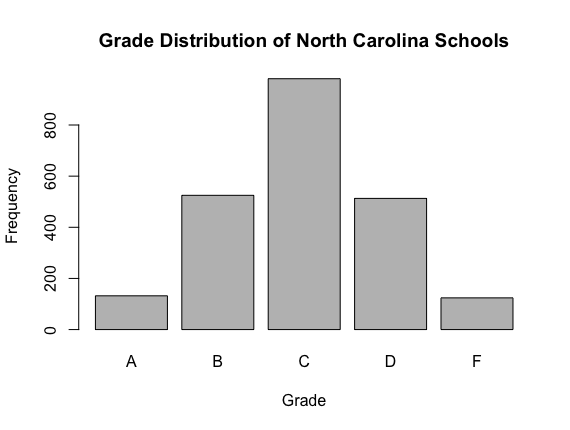
\includegraphics[scale=.37]{5ai.png}
    (a)(ii)
    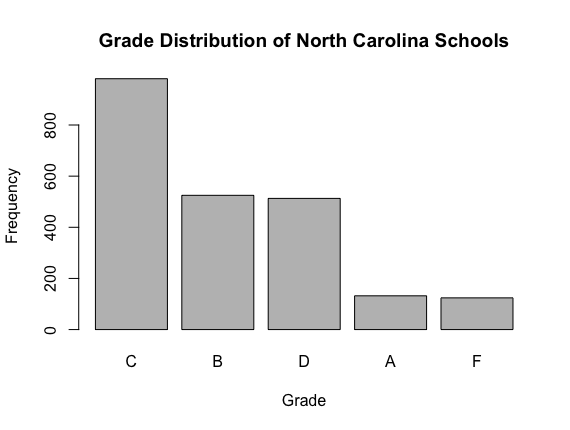
\includegraphics[scale=.37]{5aii.png}
    
    (b)(i)
    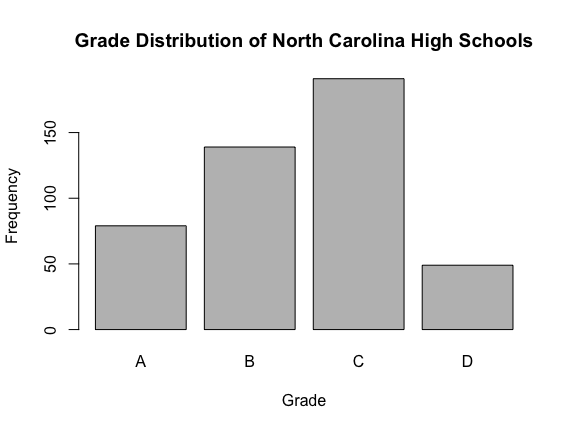
\includegraphics[scale=.37]{5bi.png}
    (b)(ii)
    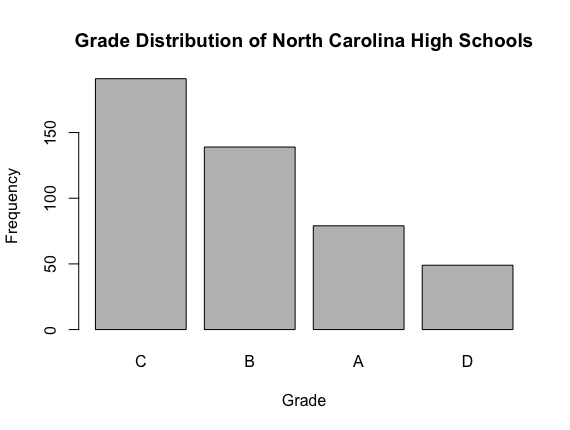
\includegraphics[scale=.37]{5bii.png}
    (b)(iii)
    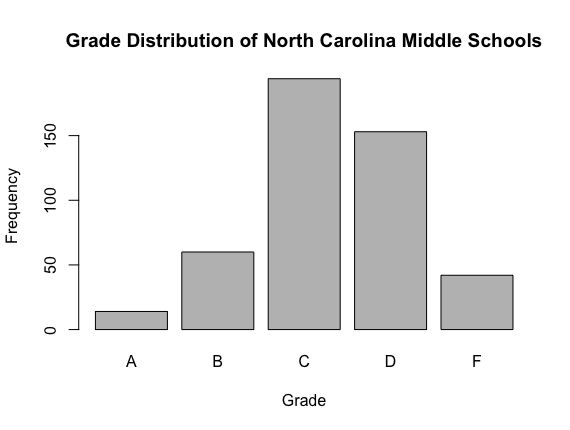
\includegraphics[scale=.37]{5biii.png}
    (b)(iv)
    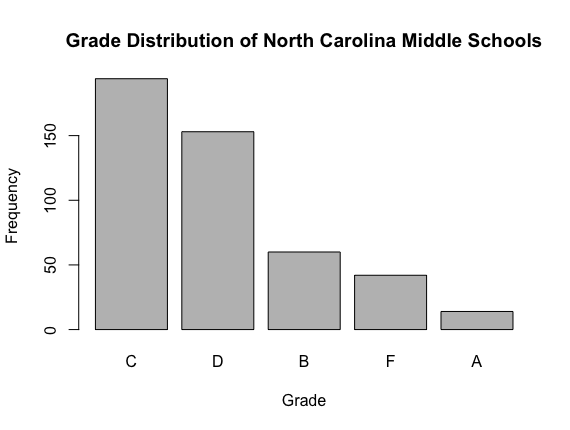
\includegraphics[scale=.37]{5biv.png}
    (b)(v)
    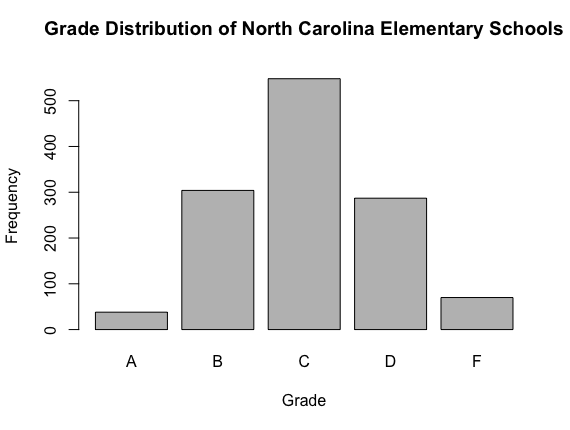
\includegraphics[scale=.37]{5bv.png}
    (b)(vi)
    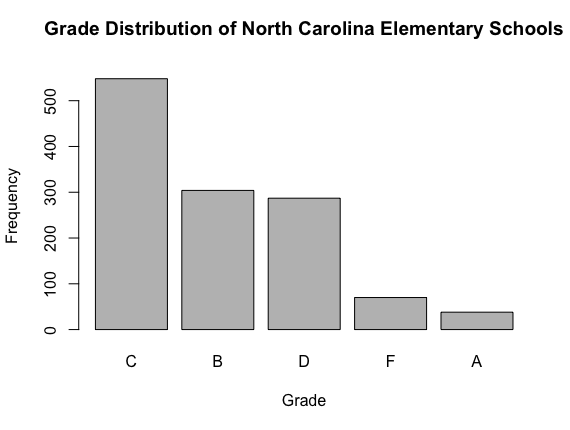
\includegraphics[scale=.37]{5bvi.png}
\end{homeworkProblem}

\begin{homeworkProblem}
    RT 1.5.5 - Maximal static inspiratory pressure (PImax) is an index of respiratory muscle strength. The following data show the measure of PImax (cm $H_2O$) for 15 cystic fibrosis patients. Do this problem by hand. Also calculate the mean and SD.\\
    \begin{enumerate}[label=(\alph*)]
    
    \item Find the lower and upper quartiles, median, and interquartile range. Check for any outliers and interpret.

    \item Construct a box plot and interpret.
    
    \item Are there any outliers?
    
    \end{enumerate}
    
    \textbf{Solution}
    \begin{enumerate}[label=(\alph*)]
    
    \item The data is given by the following sample set:
    \[S = \{105, 80, 115, 95, 100, 85, 90, 70, 135, 105, 45, 115, 40, 115, 95\}.\] The sample can be sorted to yield: \[S = \{40, 45, 70, 80, 85, 90, 95, 95, 100, 105, 105, 115, 115, 115, 135\}.\] The median for this sample is the $8^{th}$ element which is $95$. Since the sample size is $15, Q_1$ is given by the $4^{th}$ element and $Q_3$ is given by the  Thus, $Q_1 = 80, Q_3 = 115$, and IQR $= 115 - 80 = 35$. $1.5*$IQR $ = 52.5$, so the whiskers span from $Q_1 - 52.5 = 27.5$ to $Q_3 + 52.5 = 167.5$. Since the minimum of the sample is $40 \geq 27.5$ and the maximum is $135 \leq 167.5$, there are no outliers. The mean is given by 
    \[\bar{x} = \frac{1}{n}\sum_{i=1}^nx_i = \frac{40 + 45 + ... + 135}{15} = \frac{1390}{15} = \frac{278}{3}.\] The standard deviation is given by the following:
    \[SD = \sqrt{\sum_{i=1}^n\frac{(x_i - \bar{x})^2}{N}} = \sqrt{\frac{(40 - 92.667)^2 + (45 - 92.667)^2 + ... + (135 - 92.667)^2}{15}} = \sqrt{\frac{10117.86}{15}} = 25.972.\]

    \item See attached. The data indicates that there is some variance in PImax measurements for patients with cystic fibrosis, since the data is spread out across a somewhat large range, with a cluster around 40-45 and a second cluster around 115. However, the data is somewhat balanced since the median and mean are very close together.
    
    \item No. The IQR $= 115 - 80 = 35$. $1.5*$IQR $ = 52.5$, so the whiskers span from $Q_1 - 52.5 = 27.5$ to $Q_3 + 52.5 = 167.5$. Since the minimum of the sample is $40 \geq 27.5$ and the maximum is $135 \leq 167.5$, there are no outliers. 
    
    \end{enumerate}
    
\end{homeworkProblem}

\begin{homeworkProblem}
    The ncschools.csv data includes the variable, score, which is a numerical grade for school performance on a scale of 0 − 100. For each category of school (elementary, middle, high), use R to find the average, SD, min, max, and quartiles. Make a plot showing the 3 boxplots for score. Interpret the results. \\
    
    \textbf{Solution}
    For the high school category, the average score is $70.072$, the standard deviation is $12.540$, the minimum score is $43$, the maximum score is $99$, the median is $69$ and the lower and upper quartiles are given by $61$ and $78$, respectively. \\
    
    For the middle school category, the average score is $57.220$, the standard deviation is $13.242$, the minimum score is $23$, the maximum score is $96$, the median is $57$ and the lower and upper quartiles are given by $48$ and $66$, respectively. \\
    
    For the elementary school category, the average score is $61.246$, the standard deviation is $12.737$, the minimum score is $23$, the maximum score is $94$, the median is $62$ and the lower and upper quartiles are given by $53$ and $70$, respectively. \\
    
    This data indicates that high schools generally have better scores, with slightly lower variance than other categories of schools. Middle schools have a large variance, with few outliers, and are on the lower end of the score spectrum. Elementary schools are closer to the average, but still exhibit a high variance.  \\
    
    Three box plots showing the score distribution of each category of North Carolina schools is displayed below.
    
    \centerline{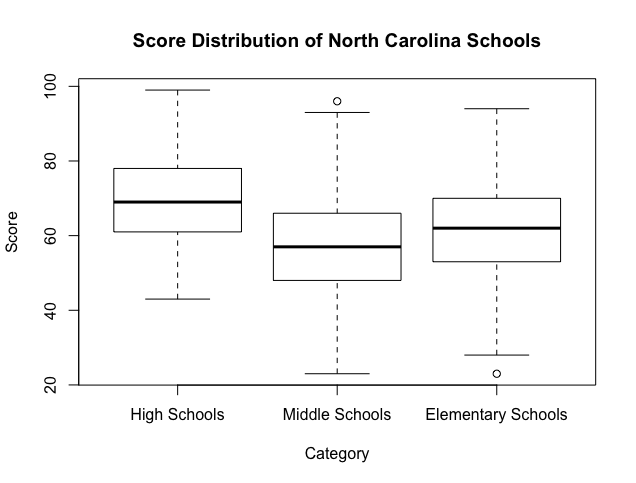
\includegraphics[scale=.37]{boxplot.png}}
\end{homeworkProblem}

\begin{homeworkProblem}
    Let $x_1, . . . , x_n$ represent a sample of $n$ observations. Show that sum of deviations from the mean is zero:
    \[\sum_{i=1}^{n}(x_i - \bar{x}) = 0.\]
    
    
    Confirm the result by hand with exercise RT 1.5.12, part B (only). \\

    
    \textbf{Solution}
    We can first consider the individual sums, and reduce the problem to 
     \[\sum_{i=1}^{n}x_i - \sum_{i=1}^{n}\bar{x} = 0 \implies \sum_{i=1}^{n}x_i = \sum_{i=1}^{n}\bar{x}. \]
     
    Then, we have:
    
    \[\begin{split}
                \sum_{i=1}^{n}x_i &= \sum_{i=1}^{n}\bar{x}
                \\
                &= \bar{x}\sum_{i=1}^{n}1
                \\
                &= n\bar{x}
                \\
                &= n\frac{1}{n}\sum_{i=1}^{n}x_i
                \\
                &= \sum_{i=1}^{n}x_i
        \end{split}\]
        
    \begin{enumerate}[label=(\alph*)]
        \item Using the data given in Exercise 1.5.12, we observe that \[\sum_{i=1}^{n} = 40+46+40+54+18+45+34+60+39+42 = 418\]. Thus, $\bar{x} = \frac{1}{n}\sum_{i=1}^{n}x_i = \frac{1}{10}418 = 41.8.$ Now, we show that \[\sum_{i=1}^{n}(x_i - \bar{x}) = 40 - 41.8 + 46 - 41.8 + 40 - 41.8 +...+ 42 - 41.8 = 418 - 10*41.8 = 0.\]
    \end{enumerate}
     
\end{homeworkProblem}

\begin{homeworkProblem}
    RT 1.5.8 - Given the sample values $x_1, x_2, ..., x_n$, show that:
    
    \[\sum_{i=1}^{n}(x_i - \bar{x})^2 = \sum_{i=1}^{n}x_i^2 - \frac{(\sum_{i=1}^n x_i)^2}{n}.\]
    
    \begin{enumerate}[label=(\alph*)]
    
    \item Verify this result for the data given in Exercise 1.5.5.
    
    \end{enumerate}
    
    \textbf{Solution}
    Using the definition of the mean, which implies that $\sum_{i=1}^{n}x_i = n\bar{x}$, we have:
    \[
        \begin{split}
                \sum_{i=1}^{n}x_i^2 - \frac{(\sum_{i=1}^n x_i)^2}{n}
                &= \sum_{i=1}^{n}(x_i - \bar{x})^2
                \\
                &= \sum_{i=1}^{n}(x_i^2 - 2x_i\bar{x} + \bar{x}^2)
                \\
                &= \sum_{i=1}^{n}x_i^2 - \sum_{i=1}^{n}2x_i\bar{x} + \sum_{i=1}^{n}\bar{x}^2
                \\
                &= \sum_{i=1}^{n}x_i^2 - \sum_{i=1}^{n}2x_i\bar{x} + n\bar{x}^2
                \\
                &= \sum_{i=1}^{n}x_i^2 - 2\bar{x}\sum_{i=1}^{n}x_i + n\bar{x}^2.
                \\
                &= \sum_{i=1}^{n}x_i^2 - 2n\bar{x}^2 + n\bar{x}^2.
                \\
                &= \sum_{i=1}^{n}x_i^2 - n\bar{x}^2
                \\
                &= \sum_{i=1}^{n}x_i^2 - \frac{(n\bar{x})^2}{n}
                \\
                &= \sum_{i=1}^{n}x_i^2 - \frac{(\sum_{i=1}^n x_i)^2}{n}
        \end{split}    \]
    
    \begin{enumerate}[label=(\alph*)]
        \item Using the data given in Exercise 1.5.5, we observe that \[\sum_{i=1}^{n} = 105 + 80 + 115 + 95 + 100 + 85 + 90 + 70 + 135 + 105 + 45 + 115 + 40 + 115 + 95 = 1390\]. Thus, $\bar{x} = \frac{1}{n}\sum_{i=1}^{n}x_i = \frac{1}{15}1390 = \frac{278}{3}.$ Now, we show that \[\sum_{i=1}^{n}(x_i - \bar{x})^2 = (105 - \frac{278}{3})^2 + (80 - \frac{278}{3})^2  + (115 - \frac{278}{3})^2 + ... + (95 - \frac{278}{3})^2  = \frac{28330}{3}.\] We compute the right hand side by showing \[\sum_{i=1}^{n}x_i^2 = 105^2 + 80^2 + 115^2 +...+ 95^2 = 138250\] and \[\frac{(\sum_{i=1}^n x_i)^2}{n} = \frac{1}{15}1390^2 = \frac{386420}{3}.\] Thus, the right hand side of the equation is given by \[\sum_{i=1}^{n}x_i^2 - \frac{(\sum_{i=1}^n x_i)^2}{n} = \frac{138250*3 - 386420}{3} = \frac{28330}{3}\]. This equality holds for the data given in Exercise 1.5.12.
    \end{enumerate}

    
\end{homeworkProblem}


\end{document}
